\documentclass[9pt]{beamer}
\usepackage{kotex}
\usepackage{amsfonts,amssymb,amsthm}
\usepackage[dvipsnames]{xcolor}
\usepackage{xcolor}
\usepackage{etoolbox}
\usepackage{braket}
\usepackage{qcircuit}

%## color
\definecolor{customBlack}{HTML}{3B4252}
\definecolor{customBlackGrey}{HTML}{434C5e}
\definecolor{cuatomGrey}{HTML}{4C566A} 
\definecolor{customWhite}{HTML}{ECEFF4} 
\definecolor{customBlue}{HTML}{6082B6}  
\definecolor{customRed}{HTML}{BF616A}
\definecolor{vividauburn}{rgb}{0.58, 0.15, 0.14}


%## Theme & custom
% \usetheme{metropolis}           % Use metropolis theme
% \metroset{block=fill}
\usetheme{moloch} % modern fork of the metropolis theme
\molochset{block=fill}
\setbeamersize{text margin left=5mm, text margin right=5mm}
\setbeamercolor{palette primary}{bg=customBlack}
\setbeamercolor{alerted text}{fg=customRed}
\setbeamercolor{itemize item}{fg=customBlue}
\setbeamercolor{enumerate item}{fg=customBlue}


%## font
\usefonttheme[onlymath]{serif}
% \setbeamerfont{normal text}{size=\small}
% \setbeamerfont{math text}{size=\tiny}


%## Theorem title, numbering
\makeatletter
\setbeamertemplate{theorem begin}
{%
\begin{\inserttheoremblockenv}
{%
\inserttheoremheadfont
\inserttheoremname
\ifx\inserttheoremaddition\@empty\else\ of\ \inserttheoremaddition\fi%
\inserttheorempunctuation
}%
}
\setbeamertemplate{theorem end}{\end{\inserttheoremblockenv}}
\makeatother
\setbeamertemplate{theorems}[numbered]  


%## Custom block
\setbeamercolor{block title}{bg=customBlue, fg=white}
\setbeamercolor{block body}{bg=customWhite, fg=customBlack}
\setbeamercolor{block title alerted}{%
    use={block title, alerted text},
    bg=customRed,
    fg=white
}
\setbeamercolor{block body alerted}{%
    use={block title, alerted text},
    bg=customWhite,
    fg=customBlack
}
\AtBeginEnvironment{definition}{%
    \setbeamercolor{block title}{fg=white,bg=customBlackGrey}
    \setbeamercolor{block body}{fg=customBlack, bg=customWhite}
}
\AtBeginEnvironment{theorem}{%
    \setbeamercolor{block title}{fg=white,bg=customBlackGrey}
    \setbeamercolor{block body}{fg=customBlack, bg=customWhite}
}
\AtBeginEnvironment{corollary}{%
    \setbeamercolor{block title}{fg=white,bg=customBlackGrey}
    \setbeamercolor{block body}{fg=customBlack, bg=customWhite}
}
\AtBeginEnvironment{lemma}{%
    \setbeamercolor{block title}{fg=white,bg=customBlackGrey}
    \setbeamercolor{block body}{fg=customBlack, bg=customWhite}
}


%! Useful command
\renewcommand{\Pr}{\text{Pr}}
% $\ast$ \underline{Proof}:
%\checkmark \underline{meaning}:

\title{7. Quantum entanglement}
\date{\today}
\author{Vaughan Sohn}
% \institute{Centre for Modern Beamer Themes}


\begin{document}
    %#################################### 
    \maketitle
    
    %#################################### 
    \begin{frame}
        \frametitle{Contents}
        \tableofcontents
    \end{frame}

    %#################################### 
    %pure state가 주어졌을 때 entangled state인지 아닌지 파악하는 방법
    \begin{section}{Entanglement in pure state}
        \begin{frame}
            \frametitle{Product state}
            Pure state에서 entanglement를 판단하는 대표적인 기준은 composite system의 state를 \textbf{product state}의 형태로 표현이 가능한지 확인하는 것이다.
            \begin{itemize}
                \item product state: $\ket{\psi}_{AB} = \ket{\psi}_A \otimes \ket{\psi}_B$
                \item entangled state: $\ket{\psi}_{AB} \ne \ket{\psi}_A \otimes \ket{\psi}_B$
            \end{itemize}
            \vspace{0.4cm}
            Example:
            \begin{itemize}
                \item 다음 state는 entangled state인가?
                \begin{equation*}
                    \frac{1}{\sqrt 2} \left ( \ket{00} + \ket{01} + \ket{10} + \ket{11} \right)
                \end{equation*}
                \item 다음 state는 entangled state인가?
                \begin{equation*}
                    \frac{1}{\sqrt 2} \left ( \ket{00} + \ket{01} + \ket{10} - \ket{11} \right)
                \end{equation*} 
            \end{itemize}
            \begin{block}{Question}
                이 방법보다 더 간단한 방법은 없을까? \\
                $\Rightarrow$ \textit{Schmidt decomposition!}
            \end{block}
        \end{frame}
        
        \begin{frame}
            \frametitle{Schmidt decomposition}
            \begin{theorem}[Schmidt decomposition]
                Schmidt decomposition은 다음과 같이 정의된다.
                \begin{equation*}
                    \ket{\psi} = \sum_{ij} c_{ij} \ket{i} \ket{j} = \sum_{k=1}^d D_{k} \ket{u_k} \ket{v_k}
                \end{equation*}
                where $\ket{\psi}_{AB} \in \mathcal H_A \otimes \mathcal H_d$, $dim(H_A \otimes H_b) = d^2$.
            \end{theorem}
            \vspace{0.4cm}
            Schmidt coefficient의 \textbf{rank}를 확인하여 entangled인지 구분할 수 있다.
            \begin{itemize}
                \item product state: $d=1$
                \item entangled state: $d>1$
            \end{itemize}
        \end{frame}

        \begin{frame}
            \frametitle{Schmidt decomposition}
            $\ast$ \underline{Proof}:\\
            \vspace{0.2cm}
            Schmidt decomposition은 다음과 같이 quantum state의 coefficient를 \alert{대각화가 가능한 $d\times d$ matrix의 원소}로 생각하는 것에서부터 출발한다.
            \begin{equation*}
                c_{ij} = [C]_{ij} = [UDV]_{ij}
            \end{equation*}
            따라서 이 표현을 대신 대입하게되면, 대각행렬 $D$의 원소들만을 사용하여 quantum state를 새로운 basis에 대해 표현할 수 있다.
            \begin{align*}
                |\psi\rangle & =\sum_{i j} [U D V]_{i j}\ket i \ket j \\
                &=\sum_{i j k} u_{i k} D_{k k} v_{k j}|i\rangle|j\rangle \\
                &=\sum_k D_k \underbrace{\sum_i u_{i k}|i\rangle}_{\left|u_k\right\rangle} \underbrace{\sum_j v_{k j}|j\rangle}_{\left|v_k\right\rangle} \\
                &=\sum_{k=1}^d D_k\left|u_k\right\rangle\left|v_k\right\rangle.
            \end{align*}
        \end{frame}

        \begin{frame}
            \frametitle{LU equivalent}
            \begin{definition}[LU equivalent]
                두 $n$-qubit state $\ket \psi$와 $\ket \phi$가 \textbf{LU equivalent}라면 다음을 만족하는 어떤 \alert{local unitary} $U_1, U_2, \cdots, U_n$가 존재한다. 
                \begin{equation*}
                    \ket{\phi} = (U_1 \otimes U_2 \otimes \cdots \otimes U_n) \ket\psi
                \end{equation*}
            \end{definition}
            \vspace{0.2cm}
            $\Rightarrow$ 만약 어떤 임의의 state $\ket{\psi}$가 product state와 LU equivalent라면 $\ket{\psi}$ \textbf{역시} product state이며, entangled state와 LU equivalent라면 $\ket{\psi}$ \textbf{역시} entangled state이다.\\\
            \vspace{0.2cm}
            
            Example: 
            \begin{itemize}
                \item LU equivalent인지 확인하고 이로부터 entangled state인지 판단하라.
                \begin{equation*}
                    \frac{1}{\sqrt 2} \left ( \ket{00} + \ket{01} + \ket{10} - \ket{11} \right), \qquad \frac{\ket{00} + \ket{11}}{ \sqrt 2}
                \end{equation*}
                \item LU equivalent인지 확인하고 이로부터 product state인지 판단하라.
                \begin{equation*}
                    \frac{1}{\sqrt 2} \left ( \ket{00} + \ket{01} + \ket{10} + \ket{11} \right), \qquad \ket{00}
                \end{equation*}
            \end{itemize}
        \end{frame}

        \begin{frame}
            \frametitle{LU equivalent and Schmidt coefficient\footnote{Schmidt rank 또한 entanglement의 양을 분석하기 위해 사용되므로 LU equivalent와 관계가 있다.}}
            \begin{block}{Note}
                만약 두 상태가 \textbf{동일한 Schmidt coefficient}를 가진다면, LU equivalent이다.
            \end{block}
            \vspace{0.2cm}
            다음과 같이 Schmidt decomposition으로 표현된 두 상태를 가정하자.
            \begin{itemize}
                \item $\ket{\psi} = D_1 \ket{00} + D_2 \ket{11}$
                \item $\ket{\phi} = D_1 \ket{uv} + D_2 \ket{u^\perp v^\perp}$
            \end{itemize}
            \vspace{0.2cm}
            그렇다면, 다음의 unitary가 존재함을 쉽게 추측할 수 있다.
            \begin{itemize}
                \item $U \ket{u} = \ket 0, U\ket{u^\perp} = 1$
                \item $V \ket{v} = \ket 0, V\ket{v^\perp} = 1$
            \end{itemize}
            \vspace{0.2cm}
            따라서 두 상태는 LU equivalent이다.
            \begin{equation*}
                \ket{\psi} = (U \otimes V) \ket{\phi}
            \end{equation*}
        \end{frame}


        \begin{frame}
            \frametitle{Reduced state and LU equivalent}
            (recap) Composite system은 \textbf{partial trace}를 이용하여 각 composed system에 대한 reduced state를 나타낼 수 있다.
            \begin{itemize}
                \item $\rho^A = \text{tr}_B [\rho^{AB}] = \sum_i \bra i_B \rho^{AB} \ket i_B$
                \item $\rho^B = \text{tr}_A [\rho^{AB}] = \sum_i \bra i_A \rho^{AB} \ket i_A$
            \end{itemize}
            \vspace{0.4cm}
            LU equivalent한 다음 두 상태를 가정하자.
            \begin{itemize}
                \item $\ket{\psi} = D_1 \ket{00} + D_2 \ket{11}$
                \item $\ket{\phi} = D_1 \ket{uv} + D_2 \ket{u^\perp v^\perp}$
            \end{itemize}
            \begin{equation*}
                \ket{\psi} = (U \otimes V) \ket{\phi}
            \end{equation*}

            \vspace{0.2cm}
            각 상태에 대해 reduced state를 구하면, 다음과 같다.
            \begin{equation*}
                \ket{\psi} = \begin{cases}
                    \rho^A_\psi = D_1^2 \ket 0 \bra 0 + D_2^2 \ket 1 \bra 1\\
                    \rho^B_\psi = D_1^2 \ket 0 \bra 0 + D_2^2 \ket 1 \bra 1
                \end{cases},\quad \ket{\phi} = \begin{cases}
                    \rho^A_\phi = D_1^2 \ket u \bra u + D_2^2 \ket {u^\perp} \bra {u^\perp}\\
                    \rho^B_\phi = D_1^2 \ket v \bra v + D_2^2 \ket {v^\perp} \bra {v^\perp}
                \end{cases}
            \end{equation*}
            $\Rightarrow$ Spectral decomposition으로 표현된 $\rho^A, \rho^B$가 동일한 eigenvalue($\lambda_i \triangleq D_i^2$)를 가지는 것을 알 수 있다.\footnote{$\rho^A_\psi, \rho^B_\psi$는 완전히 equivalent한 state, $\rho^A_\phi, \rho^B_\phi$는 Schmidt coefficient가 동일하므로 LU equivalent.}
        \end{frame}

        \begin{frame}
            \frametitle{Example}
            다음 state가 entangled state인지 아닌지 다양한 방법\footnote{product, Schmidt decomposition, LU-equivalent}으로 해결해보자.
            \begin{itemize}
                \item Example 1:
                \begin{equation*}
                    \frac{1}{\sqrt 2} \left ( \ket{00} + \ket{01} + \ket{10} + \ket{11} \right)
                \end{equation*}
                \item Example 2:
                \begin{equation*}
                    \frac{1}{\sqrt 3} \left ( \ket{00} + \ket{01} + \ket{10} \right)
                \end{equation*}
            \end{itemize}
        \end{frame}

        \begin{frame}
            \frametitle{Example}
            (Example 2) LU equivalent와 reduced matrix를 이용하여 해결하는 solution:\\
            주어진 state가 다음과 같이 Schmidt decomposition으로 표현할 수 있다고 하자.
            \begin{equation*}
                \ket{\psi} = \frac{1}{\sqrt 3}(\ket{00} + \ket{01} + \ket{10}) = \sum_k D_k \ket{u_k} \ket{v_k}
            \end{equation*}
            그러면 각각의 system $A, B$에 local operator를 가하여 동일한 basis $\{\ket k\}$로 나타낼 수 있으며, 이 state와는 LU-equivalent 관계이다.
            \begin{equation*}
                \ket{\psi'} = \sum_k D_k \ket{k} \ket{k} = (U \otimes V) \ket{\psi}
            \end{equation*}
            $\ket{\psi}$에 대한 reduced state는 각각 다음과 같다.
            \begin{equation*}
                \rho^A = \sum D_k^2 \ket{u_k} \bra{u_k} = U\left(\sum_k D_k^2 \ket{k} \bra{k}\right)U^\dagger
            \end{equation*}
            \begin{equation*}
                \Rightarrow \rho^A = \frac{2}{3} \ket + \bra + + \frac{1}{3} \ket 0 \bra 0= U\begin{pmatrix} \lambda_1 & 0 \\ 0 & \lambda_2 \end{pmatrix}U^\dagger
            \end{equation*}
            이때, $\lambda_1 > 0$, $\lambda_2 > 0$이므로 $\ket{\psi}$는 entangled state이다.$\Box$
        \end{frame}

        \begin{frame}
            \frametitle{Canonical form of Two-qubit state}
            Schmidt decomposition을 이용하면 canonical form을 정의할 수 있다.
            \begin{definition}[Canonical form of two-qubit state]
                다음과 같이 표현되는 two-qubit state는 어떤 two-qubit state $\ket{\varphi}$와도 LU-equivalent하도록 만드는 coefficient $\alpha, \beta$를 가진다.
                \begin{align*}
                    \ket \psi &= \alpha \ket{00} + \beta \ket{11}\\
                                &= \cos \theta \ket{00} + \sin \theta \ket{11},\qquad (0 \le \theta \le \pi/4)
                \end{align*}
            \end{definition}
            \vspace{0.4cm}
            $\ast$ (why?) : $\{\ket0, \ket 1\}$은 single qubit state의 대표적인 basis이며, 위의 canonical form은 대표적인 basis를 이용한 Schmidt decomposition의 형태이다.\\
            \vspace{0.2cm}
            \textit{Local unitary}를 이용하면 어떤 형태의 Schmidt decomposition이든 위와 같은 형태로 변환시킬 수 있기 때문에, 어떠한 상태와도 LU-equivalent 할 수 있다.
            \begin{itemize}
                \item $\ket{u_1} = U\ket{0},\quad \ket{u_2} = U\ket{1}$
                \item $\ket{v_1} = V\ket{0},\quad \ket{v_2} = V\ket{1}$
            \end{itemize}
            \vspace{0.2cm}
            \begin{equation*}
                \ket \varphi =  \alpha \ket{u_1v_1} + \beta \ket{u_2 v_2} = (U \otimes V)(\alpha \ket{00} + \beta \ket{11}) \approx^{LU} \ket{\psi}
            \end{equation*}
        
        \end{frame}
    \end{section}
    
    %#################################### 
    %mixed state가 주어졌을 때 entangled state인지 아닌지 파악하는 방법
    \begin{section}{Entanglement in mixed state}
        \begin{frame}
            \frametitle{Separable state}
            Mixed state에서 entanglement를 판단하는 대표적인 기준은 composite system의 density matrix가 \textbf{separable state}의 형태로 표현이 가능한지 확인하는 것이다.
            \begin{definition}[Separable state]
                A separable state can be prepared by LOCC(Local Operation and Classical Communication)
                \begin{equation*}
                    \rho^{AB} = \sum_i p(i) \left( \rho_i^A \otimes \rho_i^B \right)
                \end{equation*}
                \begin{itemize}
                    \item LO: 각 system $A$, $B$에서 $\rho_i$를 준비하기 위해 사용하는 연산
                    \item CC: mixed state의 확률분포 $\sim p$를 공유하기 위한 communication\footnote{TODO: $A$, $B$가 각각 $p(i)$의 확률로 $\rho_i^A$를 준비하는게 맞는지 확인 필요}
                \end{itemize}
            \end{definition}
        \end{frame}
        
        \begin{frame}
            \frametitle{Non-separable state: entangled state}
            \begin{definition}[Non-separable state]
                A separable state cannot be prepared by LOCC
                \begin{equation*}
                    \rho^{AB} \ne \sum_i p(i) \left( \rho_i^A \otimes \rho_i^B \right)
                \end{equation*}
                \vspace{-0.2cm}
            \end{definition}
            \begin{itemize}
                \item Example 1 : $\epsilon$이 1에 가까울수록 separable state에 가까워 짐.\footnote{$I/4$가 separable이므로}
                \begin{equation*}
                    \rho = (1-\epsilon) \ket{\psi_{ent}} \bra{\psi_{ent}} + \epsilon \  \frac{I}{4}
                \end{equation*}
                \item Example 2 :
                \begin{equation*}
                    \rho = \frac{1}{2} \ket{00} \bra{00} +  \frac{1}{2} \ket{11} \bra{11}
                \end{equation*}
                \begin{equation*}
                    \text{(sol.)}\quad  \rho=\frac{1}{2}(|0\rangle\langle 0| \otimes|0\rangle\langle 0|)+\frac{1}{2}(|1\rangle\langle 1| \otimes|1\rangle\langle 1|)
                \end{equation*}
                \item Example 3\footnote{부호가 다른 두 entanglement state들의 mixed state라서 product로 표현할 수 없는 state들이 소거된다.} : 
                \begin{equation*}
                    \rho = \frac{1}{2} \ket{\Phi^+} \bra{\Phi^+} +  \frac{1}{2} \ket{\Phi^-} \bra{\Phi^-}
                \end{equation*}
                \begin{equation*}
                    \text{(sol.)}\quad  \rho=\frac{1}{2}(|0\rangle\langle 0| \otimes|0\rangle\langle 0| + |1\rangle\langle 1| \otimes|1\rangle\langle 1|)
                \end{equation*}
            \end{itemize}
            
        \end{frame}

        \begin{frame}
            \frametitle{Example}
            \begin{itemize}
                \item Example 4 : 
                \begin{equation*}
                    \rho = \frac{1}{4} \left( \ket{\Phi^+} \bra{\Phi^+}  +  \ket{\Phi^-} \bra{\Phi^-}  + \ket{\Psi^+} \bra{\Psi^+}  +  \ket{\Psi^-} \bra{\Psi^-} \right)
                \end{equation*}
                \item Example 5 :
                \begin{equation*}
                    \rho = \frac{1}{3} \left( \ket{\Phi^+}\bra{\Phi^+} + \ket{\Phi^-} \bra{\Phi^-} + \ket{\Psi^+} \bra{\Psi^+} \right)
                \end{equation*}
            \end{itemize}
        \end{frame}

        \begin{frame}
            \frametitle{PPT Criteria}
            Mixed state의 entanglement를 확인하는 또 하나의 방법을 바로 \textbf{PPT Criteria}라고 한다. 
            \begin{theorem}[Positive Partial Transpose contidion]
                만약 $\rho$가 separable state라면, $\rho$를 이루는 system중에서 일부 system만 \alert{transpose}를 취하더라도 여전히 quantum state, 즉 \textbf{positive matrix}여야한다.
                \begin{equation*}
                    \rho^{T_B} = \sum_i p(i) \ket{e_i}\bra{e_i} \otimes \left(\ket{f_i} \bra{f_i}\right)^T \ge 0,
                \end{equation*}
                where $\rho = \sum_i p(i) \ket{e_i} \bra{e_i} \otimes \ket{f_i} \bra{f_i}$.
            \end{theorem}
            \vspace{0.2cm}
            \begin{itemize}
                \item Partial transpose: 특정 system에 대해서만 transpose를 취하는 연산
                \item Partial transpose in matrix: 
                \begin{itemize}
                    \item $T_A$: Block 1과 Block 4 내부의 요소가 각각 전치된다.
                    \item $T_B$: Block 2와 Block 3 내부의 요소가 각각 전치된다.
                \end{itemize}
                \begin{equation*}
                    \rho =
                    \begin{bmatrix}
                    \text{Block 1 (00)} & \text{Block 2 (01)} \\
                    \text{Block 3 (10)} & \text{Block 4 (11)}
                    \end{bmatrix}
                \end{equation*}
                \item Positive matrix: non-negative eigenvalue만을 가지는 행렬
            \end{itemize}
            
        \end{frame}

        \begin{frame}
            \frametitle{Example}
            Example 1 (Bell state) : \\
            $\rho = \ket{\Phi^+} \bra{\Phi^+}$의 matrix representation은 다음과 같다.
            \begin{equation*}
                \rho = \ket{\Phi^+} \bra{\Phi^+} = \frac{1}{2} \begin{pmatrix}
                    1 & 0 & 0 & 1 \\
                    0 & 0 & 0 & 0 \\
                    0 & 0 & 0 & 0 \\
                    1 & 0 & 0 & 1
                \end{pmatrix}, \qquad \text{eig}(\rho) : 1/2, 0
            \end{equation*}
            반면, 이 state의 partial transpose는 다음과 같이 \textbf{negative eigenvalue}를 가지기 때문에 entangled state이다.
            \begin{equation*}
                \rho^{T_B} = \frac{1}{2} \begin{pmatrix}
                    1 & 0 & 0 & 0 \\
                    0 & 0 & 1 & 0 \\
                    0 & 1 & 0 & 0 \\
                    0 & 0 & 0 & 1
                \end{pmatrix}, \qquad \text{eig}(\rho) : -1/2, 1/2
            \end{equation*}
        \end{frame}

        \begin{frame}
            \frametitle{Example}
            Example 2 : \\
            다음과같이 Bell state와 pure state의 mixed state로 표현된 $\rho$를 $p$가 얼마일때를 기준으로 entangled / separable state로 나뉘는가?
            \begin{equation*}
                \rho_p = (1-p) \ket{\Phi^+}\bra{\Phi^+} + p \frac{I}{4}
            \end{equation*}
            $\Rightarrow$ (hint) 기준이 되는 지점은 partial trace의 \textit{minimum eigenvalue}가 음수가 되는 지점!
            \begin{equation*}
                \rho^{T_B} = (1-p) \underbrace{\left(\ket{\Phi^+}\bra{\Phi^+}\right)^{T_B}}_{\lambda_{\min} = -1/2} + p \underbrace{\left(\frac{I}{4}\right)^{T_B}}_{\lambda_{\min} = 1/4}
            \end{equation*}
            따라서 minimum eigenvalue로부터 얻은 기준은 $\boxed{p=2/3}$ 이다.
            \begin{align*}
                \lambda^\ast &= \min_{i} \braket{v_i|\rho^{T_B} | v_i} \\
                            &= (1-p) \left(-\frac{1}{2}\right) + \frac{p}{4} < 0
            \end{align*}
        \end{frame}
    \end{section}

    \begin{frame}
        \frametitle{Summary: condition of entanglement}
        \begin{block}{Summary}
            \begin{itemize}
                \item pure state
                \begin{itemize}
                    \item (definition) product state인지 아닌지 확인한다.
                    \begin{equation*}
                        \text{(sep)} \qquad \ket{\psi}^{AB} = \ket{\psi}^A \otimes \ket{\psi}^B
                    \end{equation*}
                    \item Schmidt decomposition : rank = 1이라면 product, rank $>$ 1이라면 entangled.
                    \item Product state와 LU-equivalent라면 product, entangled state와 LU-equivalent라면 entangled.
                    \item Reduced state의 Schmidt rank = 1이라면 product, rank $>$ 1이라면 entangled.\footnote{확인 필요}
                \end{itemize}
                \item mixed state
                \begin{itemize}
                    \item (definition) separable state인지 아닌지 확인한다.
                        \begin{equation*}
                            \text{(sep)} \qquad \rho^{AB} = \sum_i p(i) \rho_i^A \otimes \rho_i^B
                        \end{equation*}
                    \item PPT Criteria : partial trace가 positive라면 separable, positive가 아니라면 entangled.
                \end{itemize}
            \end{itemize}
        \end{block}
    \end{frame}

    %#################################### 
    %entanglement의 양을 나타내는 방법
    \begin{section}{Quantity of the entanglement}
        \begin{frame}
            \frametitle{Idea of entanglement measure}
            \textbf{System} : 다음의 2-qubit quantum state\footnote{canonical form}에
            \begin{equation*}
                \ket{\psi} = \cos \theta \ket{00} + \sin \ket{11},\qquad (0< \theta < \pi/4)
            \end{equation*}
            Quantum dynamics $\mathcal E^A()$를 가하여 ($K_s$: success, $K_f$: failure (e.g., noise))
            \begin{equation*}
                \mathcal E^A(\cdot) = K_s (\cdot) K_s^\dagger +  K_f (\cdot) K_f^\dagger
            \end{equation*}
            다음의 \textit{success state}를 만들어내고자 한다고 하자.\footnote{$\mathcal E^A$는 system $A$에만 가해지는 LO이므로 entanglement를 만들어내지 못한다는 사실을 알고있다.}
            \begin{equation*}
                \ket{\Phi^+} = \frac{\ket{00} + \ket{11}}{\sqrt 2}
            \end{equation*}
            그렇다면, $\mathcal E^A()$에 대한 Kraus operator는 다음과 같이 표현된다.\footnote{(tip) $K_s$를 구하면 $K_f$는 $K$의 completeness relation으로부터 쉽게 얻을 수 있다.}
            \begin{align*}
                K_s &= a \left(\frac{\sin \theta}{\cos \theta} \ket 0 \bra 0 + \ket 1 \bra 1\right)\\
                K_f &= \sqrt{I - K_s^\dagger K_s} = \sqrt{1 - a^2 \frac{\sin^2 \theta}{\cos^2 \theta}} \ket 0 \bra 0 + \sqrt{1-a^2} \ket 1 \bra 1
            \end{align*}
        \end{frame}

        \begin{frame}
            \frametitle{Idea of entanglement measure}
            (contd.) 앞에서 정의한 $K_s, K_f$는 각각 전체 system에 다음과 같이 동작한다.
            \begin{itemize}
                \item $(K_s \otimes I)$, $a=1$일 때, 다음과 같다. 
                \begin{equation*}
                    (K_s\otimes I) \ket{\psi} = \sqrt 2 \sin \theta \frac{\ket{00} + \ket{11}}{\sqrt 2} = \sqrt 2 \sin \theta \ket{\Phi^+}
                \end{equation*}
                \item $(K_f \otimes I)$, $a=1$일 때, 다음과 같다.\footnote{product state가 되었다.}
                \begin{equation*}
                    (K_f\otimes I) \ket{\psi} = \sqrt{\frac{\cos^2 \theta - \sin^2 \theta}{\cos^2 \theta}} \ket{00}
                \end{equation*}
            \end{itemize}
            \vspace{0.2cm}
            따라서 정리하자면, quantum channel $\mathcal E^A$를 사용하여 system $A$에 LO를 가했을 때, 우리가 원하는 success state $\ket{\Phi^+}$를 만들어낼 확률은 $\boxed{2 \sin^2\theta}$이다.
            
            \vspace{0.2cm}
            만약 $\mathcal E^A(\cdot)$를 $\ket \psi$에 가하는 과정을 $N$번 수행하면, success state $\ket{\Phi^+}$는 $N \cdot 2\sin^2\theta$개가 만들어 질 것이라고 기대할 수 있다. 반면, failure state는 \alert{product state}이다.
            \begin{alertblock}{Idea of entanglement measure}
                따라서 (maximal entangled state인) $\ket{\Phi^+}$를 {entanglement}의 \textbf{단위}로 생각할 수 있다.
            \end{alertblock}
        \end{frame}

        \begin{frame}
            \frametitle{Idea of entanglement measure}
            예를 들어, 다음과 같은 서로 다른 두 상태를 가정하자.
            \begin{equation*}
                \ket{\psi_1} = \cos \theta_1 \ket{00} + \sin \theta_1 \ket{11},\qquad \ket{\psi_2} = \cos \theta_2 \ket{00} + \sin \theta_2 \ket{11}
            \end{equation*}
            각각의 상태에 $\mathcal E^A(\cdot)$를 가하는 과정을 $N$번 반복하면, 각각 $\ket{\Phi^+}$ state가 만들어진 개수는 다음과 같다.
            \begin{itemize}
                \item $\ket{\psi_1}$ : $M_1 \triangleq N \cdot 2 \sin^2 \theta_1$
                \item $\ket{\psi_2}$ : $M_2 \triangleq N \cdot 2 \sin^2 \theta_2$
            \end{itemize}
            따라서, $\ket{\Phi^+}$ state의 개수를 비교하여, 만약 $M_1 > M_2$라면 $\ket{\psi_1}$이 $\ket{\psi_2}$보다 더 entangled state라고 판단할 수 있다.
            \begin{figure}
                \centering
                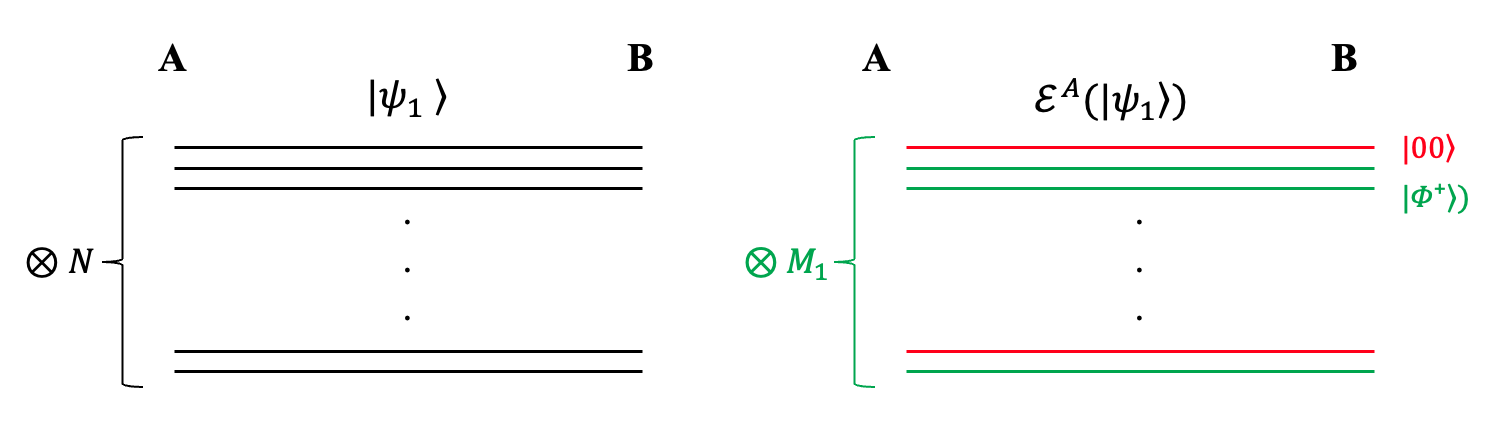
\includegraphics[width=0.9\textwidth]{image/L7_entanglement_measure_exp.png}
            \end{figure}
        \end{frame}

        \begin{frame}
            \frametitle{Entanglement measure}
            앞의 아이디어를 일반화하여, single qubit $\ket{\psi}$에만 적용하는 operation이 아니라 $N$개의 복사본으로 이루어진 $\ket{\psi}^{\otimes N}$에 적용하는 \textbf{multi-qubit} operation까지 고려해보자.\\
            \vspace{0.2cm}
            $\rightarrow$ $\ket{\psi}^{\otimes N}$에 각각의 Local Operation을 취했을 때 얻는 $\ket{\Phi^+}$ state의 개수 $M$.\footnote{TODO: 각 local operation을 취했을 때 얻어지는 $M$ 중에서 최댓값?}

            \vspace{0.4cm}
            $\ket{\psi}^{\otimes N}$ state를 전개하면 다음과 같다.
            \begin{align*}
                \ket{\psi}^{\otimes N} & = \scriptsize \left(\cos \theta \ket{00} + \sin \theta \ket{11} \right)^{\otimes N} \\
                & =  \scriptsize  \left(\cos \theta \ket{00} + \sin \theta \ket{11} \right)_{A_1B_1} \cdots \left(\cos \theta \ket{00} + \sin \theta \ket{11} \right)_{A_NB_N} \\
                & = \scriptsize   \Big(\cos^2 \theta \ket{00}_{A_1A_2} \ket{00}_{B_1B_2} + \cos\theta \sin \theta \big(\ket{01}_{A_1A_2}\ket{01}_{B_1B_2} + \ket{10}_{A_1A_2} \ket{10}_{B_1B_2}\big) \\ 
                &\quad  \scriptsize  + \sin^2 \theta \ket{11}_{A_1A_2} \ket{11}_{B_1B_2} \Big) \Big( \cos \theta \ket{00} + \sin \theta \ket{11}\Big)^{\otimes N-2} \\
                & = \scriptsize  \cos^N\theta \ket{0^n}_{A_1^n} \ket{0^n}_{B_1^N} + \cos^{N-1} \theta \sin \theta \Big(  \ket{0^{n-1} 1}\ket{0^{n-1} 1} + \ket{0^{n-2}10} \ket{0^{n-2}10}\\
                &\quad  \scriptsize  + \cdots + \ket{10^{n-1}} \ket{10^{n-1}}\Big) + \cdots + \sin^N \theta \ket{1^n} \ket{1^n}
            \end{align*}
        \end{frame}


        \begin{frame}
            \frametitle{Entanglement measure}
            (contd.) 앞에서 전개한 $\ket{\psi}^{\otimes N}$의 state에 WLLN을 적용하면, $\ket {\psi}^{\otimes N}$ state를 이루는 qubit이 다음의 분포를 따른다고 추정할 수 있다.\footnote{전개 없이도 $\ket{\psi_1}$의 canonical form에서 확률을 예측할 수 있다.}
            \begin{equation*}
                0 \sim \sin^2 \theta, \qquad 1  \sim \cos^2 \theta
            \end{equation*}
            즉, $N$ qubit에서 0의 개수와 1의 개수가 각각 다음과 같으리라고 기대할 수 있다.
            \begin{equation*}
                \# 0 = N \cdot \sin^2 \theta,\qquad \# 1 = N \cdot \cos^2 \theta
            \end{equation*}
            실제로 위와 같은 개수의 0과 1을 갖는 sequence가 바로 \textit{Typical sequence}이다.
            \begin{block}{Recap: Typical set, Typical subspace, Typical projector}
                \begin{itemize} 
                    \item Typical set : $X \sim Bern(p)$, i.i.d
                    \begin{equation*}
                        A_{\epsilon}^{(n)} = \{x_1^n \ : \ 2^{-n(H(p) + \epsilon) \le P_X(x^n) \le 2^{-n(H(p) - \epsilon)}}\}
                    \end{equation*}
                    \item Typical subspace : 
                        $ T_\epsilon^{(n)} = \text{span} \{ \ket{x_1\cdots x_n},\ : \ x_1\cdots x_n \in A_\epsilon^{(n)} \} $
                    \item Typical subspace projector : 
                        $ P_\epsilon^{(n)} = \sum_{x^n_1 \in A_\epsilon^{(n)}} \ket{x^n_1} \bra{x^n_1} $
                \end{itemize}
            \end{block}
        \end{frame}

        \begin{frame}
            \frametitle{Entanglement measure}
            (contd.) Typical subspace projector를 system $A$의 Local Operator로 가하면, 다음과 같고
            \begin{equation*}
                (P_\epsilon^{(N)} \otimes I) \ket{\psi}^{\otimes N} = \sum_{x^N_1 \in A_\epsilon^N} \sqrt{2^{-NH([\cos^2 \theta, \sin^2 \theta])}} \ket{x^N_1} \ket{x^N_1}
            \end{equation*}
            원래 상태와 typical subspace에 투영된 상태 간 distance는 $N$이 증가함에 따라 0으로 수렴한다. 
            \begin{equation*}
                \| \ket{\psi}^{\otimes N} - (P_\epsilon^{(N)} \otimes I)\ket{\psi}^{\otimes N}  \| \rightarrow 0,\qquad as\ N \rightarrow \infty
            \end{equation*}
            (아이디어) $\ket{\Phi^+}$은 \textbf{maximal entangled state}이므로, \alert{quantum compression}에서 $N$ qubit을 나타내기 위해 사용하는 random qubit으로 간주할 수 있다. 
            따라서 다음이 성립한다.
            \begin{equation*}
                \ket{\psi}^{\otimes N} \approx (P_\epsilon^{(N)} \otimes I) \ket{\psi}^{\otimes N} \approx \ket{\Phi^+}^{\otimes M},\qquad as \ N \rightarrow \infty
            \end{equation*}
            따라서 주어진 state의 entanglement measure는 다음과 같이 정의된다. 
            \begin{definition}[Entropy of entanglement]
                $N$은 $\ket{\psi}$의 개수를 의미하며 , $M$은 $\ket{\Phi^+}$의 개수를 나타낸다. 
                \begin{equation*}
                    E(\ket{\psi}) = \frac{M}{N} = S(\rho^A)
                \end{equation*}
            \end{definition}
        \end{frame}

        \begin{frame}
            \frametitle{Entanglement measure}
            반면, mixed state에 대한 entanglement measure는 다음과 같이 정의된다. 
            \begin{definition}[Entropy of entanglement on mixed state\footnote{Convex-roof constraction}]
                \vspace{-0.2cm}
                \begin{equation*}
                    E(\rho) = \inf_{\{p(i), \ket{\psi_i}\}} \sum_i p(i) E(\ket{\psi_i})
                \end{equation*}
                where $\rho = \sum_i p(i) \ket{\psi_i} \bra{\psi_i}$
            \end{definition}
            \begin{itemize}
                \item Mixed state는 pure state들의 convex combination이므로 pure state의 entropy of entanglement로 계산된다.
                \item (주의) 단, 하나의 mixed state는 다양한 방식으로 표현될 수 있기 때문에, 그 중에서 가장 작은 값(infimum)으로 정의해야한다.
            \end{itemize}

            \vspace{0.2cm}
            Example: 
            \vspace{-0.4cm}
            \begin{align*}
                \rho    &= \frac{1}{2} \ket{\Phi^+} \bra{\Phi^+} + \frac{1}{2} \ket{\Phi^-} \bra{\Phi^-} \\
                        &= \frac{1}{2} \ket{00} \bra{00} + \frac{1}{2} \ket{11} \bra{11} 
            \end{align*}
            \vspace{-0.2cm}
            \begin{itemize}
                \item (decomposition 1) $E(\ket{\Phi^+}) + E(\ket{\Phi^-}) > 0$ 
                \item (decomposition 2) $E(\ket{00}) + E(\ket{11}) = \boxed{0}.$
            \end{itemize}
        \end{frame}

        \begin{frame}
            \frametitle{Distillation of entanglement in pure state}
            
            \underline{Question 1} : 왜 $\ket{\Phi^+}$의 개수로 entanglement의 quantity를 나타내는가?
            \begin{itemize}
                \item Alice가 자신의 qubit에 아무리 LOCC를 가하더라도, LOCC는 entanglement를 만들어낼 수 없고 오히려 entanglement를 감소시킬 수 있기 때문에, LOCC를 가하여 만들어지는 각 상태들은 entanglement의 크기에 대해 "순서"를 가진다.
                \begin{equation*}
                    \{\psi_1, \ \psi_2, \cdots, \psi_n \} \ : \ \text{order structure}
                \end{equation*}
                \item 이떄, 이 상태들 중에서 가장 큰 entanglement entropy를 가지는 state가 바로 $\ket{\Phi^+}$이다! 따라서 다음 관계가 성립한다.\footnote{maximally entangled state}
                \begin{equation*}
                    \ket{\Phi^+} \xrightarrow{p=1} \ket{\psi_i}, \qquad \ket{\psi_i} \xrightarrow{p<1} \ket{\Phi^+},\qquad \forall i
                \end{equation*}
            \end{itemize}
            \vspace{0.2cm}
            \underline{Question 2} : single qubit에 대한 LO와 multiple qubit에 대한 LO가 어떻게 다른가?
            \begin{itemize}
                \item single qubit에 대한 LOCC로 만들어낼 수 있는 $\ket{\Phi^+}$의 개수는 $N \cdot 2 \sin^2 \theta$이며
                \item multiple qubit에 대한 LOCC까지 고려했을 때, $N \cdot S(\rho^A)$이다.
                \item entropy의 concavity 때문에 $S(\rho^A) > 2\cdot \sin^2 \theta$가 성립한다.
            \end{itemize}
        \end{frame}

        \begin{frame}
            \frametitle{Distillation of entanglement in mixed state}
            $A$가 bell state로 준비한 quantum state를 \textit{quantum channel} $\mathcal E(\cdot)$를 사용하여 전송한다고 하자. 이 때 system 전체에 가해지는 연산은 $I \otimes \mathcal E^B$로 표현할 수 있다. 
            \begin{figure}
                \centering
                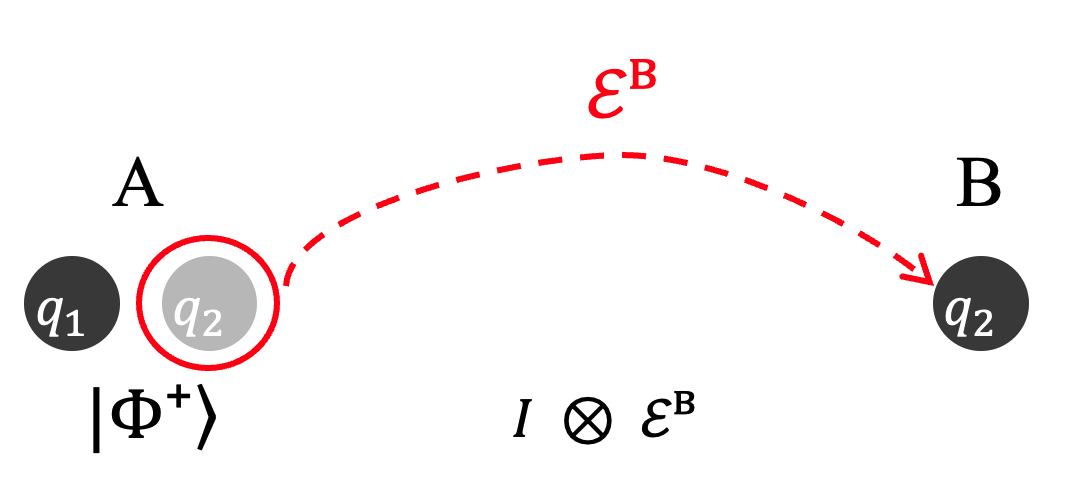
\includegraphics[width=0.55\textwidth]{image/L7_dist.png}
            \end{figure}
            \begin{equation*}
                \rho^{AB} = I \otimes \mathcal E^B(\ket{\Phi^+} \bra{\Phi^+})
            \end{equation*}
            Quantum channel을 Kraus operator로 나타냈을 때,\footnote{$\mathcal E (\cdot) = \sum_i K_i (\cdot) K_i^\dagger$} $\rho^{AB}$는 다음과 같다.
            \begin{align*}
                \rho^{AB} &= \sum_i I \otimes K_i^B \ket{\Phi^+} \bra{\Phi^+} I \otimes {K^B_i}^\dagger = \sum_i p(i) \sigma_i^{AB}
            \end{align*}
            where $p(i) \sigma_i^{AB} = (I \otimes K_i^B) \ket{\Phi^+} \bra{\Phi^+} (I \otimes K_i^B)^\dagger$
        \end{frame}

        \begin{frame}
            \frametitle{Distillation of entanglement in mixed state}
            (contd.) $\rho^{AB}$를 mixed state로 나타내기 위해서 $p(i), \sigma_i$를 계산하자.
            \begin{itemize}
                \item $p(i)$: state에 trace를 취해서 얻을 수 있다.\footnote{$I$ 생략}
                \begin{equation*}
                    p(i) = \text{tr}\left[ K_i^B \ket{\Phi^+} \bra{\Phi^+} {K_i^B}^\dagger\right]
                \end{equation*}
                \item $\sigma_i$: $p(i) \sigma_i$를 $p(i)$로 나눈다.
                \begin{equation*}
                    \sigma_i = \frac{K_i \ket{\Phi^+} \bra{\Phi^+} {K_i^B}^\dagger}{\text{tr}\left[ K_i^B \ket{\Phi^+} \bra{\Phi^+} {K_i^B}^\dagger\right]} 
                \end{equation*}
            \end{itemize}
            $\Rightarrow$ 정리하면 Alice가 $\ket{\Phi^+}$를 만들고 두 번쨰 qubit을 $B$에게 전송하여 e-bit를 공유하고자 하였지만 noisy channel 때문에 각각 $p(i)$ 확률로 $\sigma_i$라는 다른 state로 변하게 된다.
            \begin{block}{Note}
                Pure state (e.g., $\ket{\Phi^+}$)로부터 mixed state(e.g., $\rho^{AB}$)가 만들어지는 것은 physically 가능하지만, mixed state를 다시 원래 pure state로 되돌리는 것은 physically 불가능하다.
            \end{block}
        \end{frame}

        \begin{frame}
            \frametitle{Distillation of entanglement in mixed state}
            이제 다음 상황을 한번 가정해보자.
            \begin{itemize}
                \item $A$가 어떤 state를 생성하고, quantum channel을 통해 전송하여 $B$와 $\rho^{AB}$ state를 공유하고 있다. (unknown state)
                \item 위 과정을 $N$번 반복하며 얻은 $\rho^{\otimes N}$에 LOCC를 가하여 $\ket{\Phi^+}^{\otimes M}$을 만들 수 있는가?
            \end{itemize}
            \vspace{0.2cm}
            Answer: 다음과정을 거치면 가능하다. (단, 특정 probability에 따라 가능하다.)
            
            \vspace{0.1cm}
            \textbf{1. Twirling}\footnote{주어진 양자상태를 특정한 대칭성을 가진 상태로 변환하는 과정: $A$에 random unitary를 가하고 $B$에 그 unitary의 conjugation을 가하는 연산을 $n$번 수행하여 평균낸다.} : 주어진 state를 LOCC를 사용하여 다음 형태로 변환한다.
            \begin{equation*}
                \rho_F = \frac{1}{n} \sum_i (U_i \otimes U_i^*) \rho (U_i \otimes U_i^*)^\dagger
            \end{equation*}
            Isotropic state\footnote{특정 Bell state와 $I/4$ 사이의 convex combination 상태}; $\rho_F$는 다음과 같이 표현된다. (unknown parameter $p$로 표현됨)
            \begin{equation*}
                \rho_F = (1-p) \ket{\Phi^+} \bra{\Phi^+} + p \frac{I}{4}
            \end{equation*}
            isotropic state와 $\ket{\Phi^+}$간의 overlap; singlet fraction을 측정한다.
            \begin{equation*}
                F = \braket{\Phi^+ | \rho_F | \Phi^+}
            \end{equation*}

        \end{frame}

        \begin{frame}
            \frametitle{Distillation of entanglement in mixed state}
            (contd.) $F$를 계산하면 다음과 같이 $p$에 대해서 나타낼 수 있으며
            \begin{equation*}
                F = (1-p) + \frac{p}{4} = 1- \frac{3}{4} p
            \end{equation*}
            이를 이용하면 $\rho_F$를 $F$에 대해서 표현할 수 있다.
            \begin{equation*}
                \rho_F = F\ket{\Phi^+}\bra{\Phi^+} + \frac{1-F}{3} \ket{\Phi^-}\bra{\Phi^-} + \frac{1-F}{3} \ket{\Psi^+} \bra{\Psi^+} + \frac{1-F}{3} \ket{\Psi^-} \bra{\Psi^-}
            \end{equation*} 
            \vspace{0.3cm}

            따라서 $F$의 값에 따라, $\rho_F$의 state를 추측할 수 있다.
            \begin{itemize}
                \item $F=1$, $\rho_F = \ket{\Phi^+}\bra{\Phi^+}$
                \item $F=1/2$, $\rho_F$에서 $\color{red}p=2/3$이 된다. 
            \end{itemize}
            
            \begin{block}{Conclusion}
                $\rho_F$ is entangled \textit{if and only if} $F > 1/2$.
            \end{block}
            
            Twirling 과정을 거친 뒤에는 $\rho_F^\otimes N$ state를 가지게 된다.
        \end{frame}

        \begin{frame}
            \frametitle{Distillation of entanglement in mixed state}
            \textbf{2. Bilateral CNOT}을 가한다.\\
            2개의 $\rho_F$에 대해 CNOT을 가한 뒤 측정한다.\\
            \begin{figure}
                \centering
                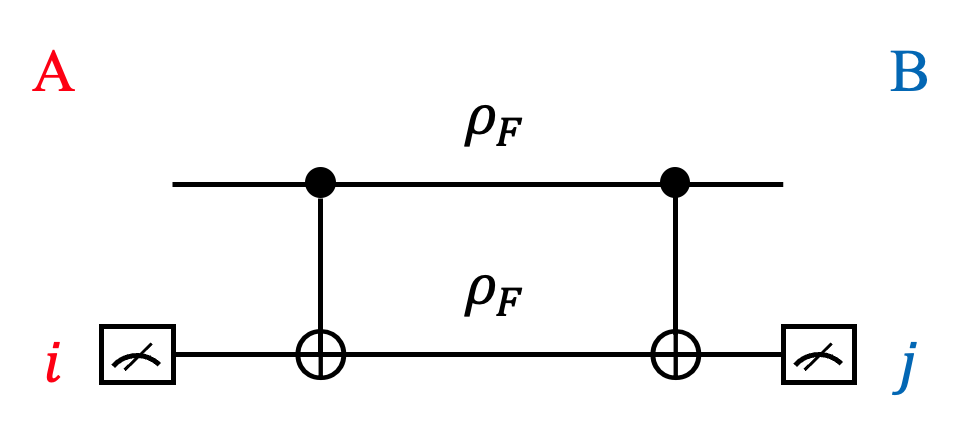
\includegraphics[width=0.45\textwidth]{image/L7_measure.png}
            \end{figure}
            \textbf{3. Classical Communication}: $A$와 $B$의 측정결과를 공유하여 다음과 같이 결정한다.
            \begin{itemize}
                \item if $i=j$: accept the first register
                \item if $i\ne j$: discard and restart
            \end{itemize}
            \textbf{4. Resulting state} $\tilde \rho_F$에 대한 $F$는 다음과 같다.
            \begin{equation*}
                F' = \braket{\Phi^+|\tilde \rho_F | \Phi^+} = \frac{F^2 + \left(\frac{1-F}{3}\right)^2}{F^2 + \frac{2}{3} F(1-F) + \frac{5}{9} (1-F)^2}
            \end{equation*}
        \end{frame}

        \begin{frame}
            \frametitle{Distillation of entanglement in mixed state}
            $F$와 $F'$의 관계를 그림으로 그리면 다음과 같다. 
            \begin{itemize}
                \item 만약 $F>1/2$라면 위의 과정을 통해 얻은 resulting state $\tilde \rho_F$에 대한 fidelity가 증가한다. (i.e., $\ket{\Phi^+}$와 더 가까운 상태가 된다.)
                \item 새로 얻은 $\tilde \rho_F$에 대해 다시 앞선 과정을 반복하면, 점차 $F'$가 증가하게 될 것이고 결국 $F=1$로 수렴하게 된다.
                \\$\Rightarrow$ $\ket{\Phi^+}$ is distilled!
            \end{itemize}
            \vspace{0.2cm}
            \begin{figure}
                \centering
                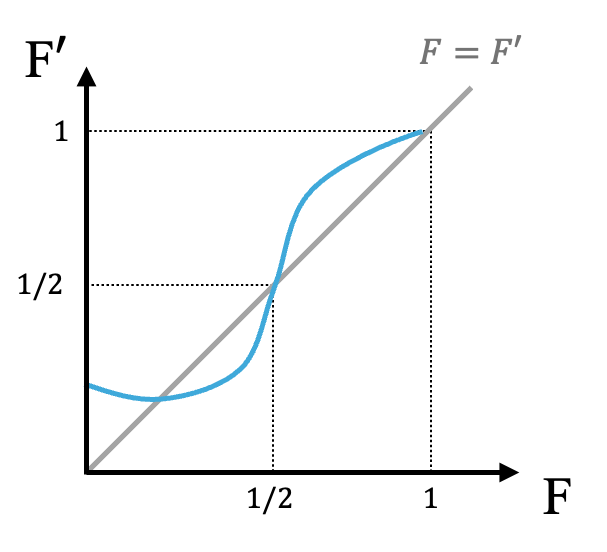
\includegraphics[width=0.4\textwidth]{image/L7_graph.png}
            \end{figure}
        \end{frame}
    \end{section}

    \begin{frame}
        \frametitle{Summary: quantuntity of entanglement}
        \begin{block}{Summary}
            \begin{itemize}
                \item Entanglement measure
                \begin{itemize}
                    \item pure state:
                    \begin{equation*}
                        E(\ket{\psi}) = S(\rho^A)
                    \end{equation*}
                    \item mixed state:
                    \begin{equation*}
                        E(\rho) = \inf_{\{p(i), \ket{\psi_i}\}} \sum_i p(i) E(\ket{\psi_i})
                    \end{equation*}
                \end{itemize}
                \item Distillation of entanglement (with LOCC)
                \begin{itemize}
                    \item pure state:
                    \begin{itemize}
                        \item single qubit LOCC: $N \cdot 2\sin^2 \theta$개의 $\ket{\Phi^+}$를 만들 수 있다.
                        \item multi-qubit LOCC: $N \cdot S(\rho^A)$개의 $\ket{\Phi^+}$를 만들 수 있다.
                    \end{itemize}
                    \item mixed state:
                    \begin{enumerate}
                        \item Twirling $\rho \rightarrow \rho_F$ 
                        \item Fidelity $F(\ket{\Phi^+}\bra{\Phi^+}, \rho)$ if $F>1/2$ can distilled.
                        \item Bilateral CNOT and measure
                        \item Classical communication, if $i=j$ accept the first register
                        \item \textit{repeat}, until $F' \rightarrow 1$. 
                    \end{enumerate}
                \end{itemize}
            \end{itemize}
        \end{block}
    \end{frame}

    %#################################### 
    %state가 어떤 state인지에 대한 정보가 없을 때 (arbitrary 안 알려진 상태) entanglement의 양을 나타내는 방법
    \begin{section}{Entanglement witness}
        \begin{frame}
            \frametitle{Entanglement witness}
            주어진 state의 정보를 알고있다면\footnote{state vector, density matrix를 표현할 수 있다면}, 앞에서 소개한 방법을 활용하여 entangled인지 아닌지 파악할 수 있다. 그렇다면, 알려지지 않은 임의의 state가 entangled인지는 어떻게 판단할 수 있을까?
            
            \vspace{0.2cm}
            $\Rightarrow$ 이를 위하여 도입된 \textit{Observable}이 바로 Entanglement witness이다.
            \begin{definition}[Entanglement witness]
                다음 2가지 조건을 만족하는 \textit{observable} $W = W^\dagger$는 entanglement witness이다.
                \begin{itemize}
                    \item $\text{tr}[W \sigma_{sep}] \ge 0$, $\forall \sigma_{sep}$ : \textbf{모든} separable state에 대해 positive trace를 가진다.
                    \item $\text{tr}[W \sigma_{ent}] < 0$, $\exists \sigma_{ent}$ : \textbf{어떤} entangled state에 대해서는 negative trace를 가진다.
                \end{itemize}
            \end{definition}
            
            \vspace{0.2cm}
            따라서 EW를 이용하면, trace positive test를 통해서 주어진 state가 entangled state인지 아닌지 확인할 수 있다. (in physical, observable $W$에 대한 측정 결과가 음수인지 양수인지 확인하는 것)
            \begin{block}{Trace positive test}
                \begin{itemize}
                    \item If $\text{tr} [W\rho] < 0$, then $\rho$ is \textbf{must} entangled state.
                    \item If $\text{tr} [W\rho] \ge 0$, then $\rho$ is product of entangled state. (not sure)
                \end{itemize}    
            \end{block}
        \end{frame}
        
        \begin{frame}
            \frametitle{Entanglement witness}
            Example: 다음 $W$가 Entanglement witness의 조건을 만족하는지 확인하라.
            \begin{equation*}
                W = \frac{1}{2} I \otimes I - \ket{\Phi^+} \bra{\Phi^+}
            \end{equation*}
            \vspace{-0.2cm}
            \begin{block}{Idea}
                $\arg\min_{\sigma_{sep}} \text{tr}[W \sigma_{sep}]$에 대해서도 여전히 trace가 positive임을 보일 수 있다면 첫 번째 조건을 만족함을 알 수 있다.
            \end{block}
            $\sigma_{sep}$이 separable state라면, 정의에 의하여 다음과 같이 표현할 수 있다.
            \begin{equation*}
                \sigma_{sep} \sum_i p(i) \ket{e_if_i} \bra{e_if_i}
            \end{equation*}
            따라서 positive trace test는 다음과 같이 기술된다.
            \begin{align*}
                \min_{\rho_{sep}} \text{tr}[W\sigma_{sep}] &= \min_{\{p(i),\ket{e_if_i}\}} \sum_i p(i) \text{tr}[W \ket{e_if_i} \bra{e_if_i}] \\
                &\ge \min_{\ket{ef}} \text{tr}[W \ket{ef} \bra{ef}]\\
                &=\frac{1}{2} - \max_{\ket{ef}} |\braket{\Phi^+|ef}|^2 = \frac{1}{2} - \frac{1}{2} = \boxed{0}
            \end{align*}
            따라서 모든 separable state에 대해 minimum trace가 0이므로 첫 번째 조건을 만족한다.
        \end{frame}
        
        \begin{frame}
            \frametitle{Feasibleness}
            그럼 실제 physically, Entanglement witness를 이용한 test를 어떻게 설계해야할까?
            \begin{equation*}
                W = \frac{1}{2} I \otimes I - \ket{\Phi^+} \bra{\Phi^+}
            \end{equation*}

            $I/2$는 constant이므로 $\ket{\Phi^+} \bra{\Phi^+}$를 구현해야한다.\\
            $\rightarrow$ \alert{Bell basis에서의 측정}으로 구현할 수 있지만, Bell basis의 측정은 비싸다.\footnote{H, CNOT를 computational basis measurement전에 가해줘야한다.}
            
            \vspace{0.2cm}
            (아이디어) Bell basis는 Pauli observable, 즉 \textit{local observable}들로 표현할 수 있다.
            \begin{align*}
                \ket{\Phi^+}\bra{\Phi^+} = \frac{1}{4} \left( I\otimes I + Z\otimes Z + X \otimes X - Y \otimes Y \right) \\
                W = \frac{1}{4} \left( I \otimes I - X \otimes X + Y \otimes Y - Z \otimes Z \right)
            \end{align*}
            이를 positive trace test에 대입하면, 다음과 같이 각각의 \alert{local observable에 대한 측정결과의 기댓값의 합}으로 표현할 수 있다는 것을 알 수 있다.
            \begin{equation*}
                \text{tr}[W \rho] = \frac{1}{4}\bigg(\underbrace{\text{tr} [II\rho]}_{=1} - \text{tr} [XX\rho] + \text{tr} [YY\rho] - \text{tr} [ZZ\rho] \bigg)
            \end{equation*}
        \end{frame}

        \begin{frame}
            \frametitle{Feasibleness}
            따라서 각각의 Pauli observable은 다음과 같이 자신에 대응되는 basis를 이용하여 측정한 결과를 사용하여 표현할 수 있다.\footnote{$\ket{+-}$와 같은 상태의 측정은 첫번째 measurement는 $\ket +$이고 두번쨰 measurement는 $\ket -$인 상황}
            \begin{align*}
                \text{tr}[XX \rho] &= \text{tr}\Big[\Big(\ket{++} \bra{++} + \ket{--} \bra{--} - \ket{+-} \bra{+-} - \ket{-+}\bra{-+}\Big)\rho\Big] \\
                    &= p(++) + p(--) - p(+-) - p(-+)
            \end{align*}
            마찬가지로 다른 Pauli observable의 기댓값도 구할 수 있다.
            \begin{block}{Note}
                $W$는 local observable들로 decomposition 할 수 있기 때문에 실험적으로 구현할 수 있다. \\
                $\longrightarrow$ \textit{feasible!}
            \end{block}
        \end{frame}
        
        \begin{frame}
            \frametitle{Example}
            Example: 다음 state가 entangled state가 되는 $p$를 EW를 사용하여 구해보자.
            \begin{equation*}
                \rho = p \frac{I}{4} + (1-p) \ket{\Phi^+} \bra{\Phi^+}
            \end{equation*}
            EW에 대한 trace는 다음과 같다.
            \begin{align*}
                \text{tr}[W \rho] &= \text{tr}\left[\left(\frac{1}{2} I \otimes I - \ket{\Phi^+}\bra{\Phi^+}\right)\rho\right] \\
                                    &= \frac{1}{2} - \text{tr}[\ket{\Phi^+} \bra{\Phi^+} \rho]\\
                                    &= \frac{1}{2} - \left(\frac{1}{4}p + (1-p)\right)
            \end{align*}
            따라서 이 trace가 음수가 되기 위한 $p$는 다음과 같이 구해진다. $\Box$
            \begin{equation*}
                \frac{1}{2} < 1 -\frac{3}{4}p \quad \Rightarrow \quad p < \frac{2}{3}.
            \end{equation*}
        \end{frame}
    \end{section}

    \begin{frame}
        \frametitle{Summary: entanglement witness of arbitrary quantum state}
        \begin{block}{Summary}
            \begin{itemize}
                \item Entanglement witness :
                다음 2가지 조건을 만족하는 \textit{observable} $W = W^\dagger$는 entanglement witness이다.
                \begin{itemize}
                    \item $\text{tr}[W \sigma_{sep}] \ge 0$, $\forall \sigma_{sep}$ : \textbf{모든} separable state에 대해 positive trace를 가진다.
                    \item $\text{tr}[W \sigma_{ent}] < 0$, $\exists \sigma_{ent}$ : \textbf{어떤} entangled state에 대해서는 negative trace를 가진다.
                \end{itemize}
                \item Entangled test:
                \begin{itemize}
                    \item 만약 trace가 negative라면 $\rho$는 확실히 entangled state이다.
                    \item 만약 trace가 positive라면 $\rho$는 product 또는 entangled state이다.
                \end{itemize}
            \end{itemize}
        \end{block}
    \end{frame}

    %#################################### 
    \begin{section}{General theory of  Entanglement witness}
        \begin{frame}
            \frametitle{Convexity on separable state set}
            서로 다른 두 state의 convex combination을 생각해보자.
            \begin{equation*}
                \sigma = (1-p) \sigma_1 + p \sigma_2,\qquad (0 \le p \le 1)
            \end{equation*}
            \vspace{-0.2cm}
            \begin{itemize}
                \item separable state의 convex combination으로 정의된 state는 \textbf{여전히 separable state}
                \item separable state와 entangled state의 convex combination으로 정의된 state는 $p$의 값에 따라서 entangled or separable이 결정된다. (using EW)
                \item entangled state의 convex combination으로 정의된 state는 \textbf{entangled state}가 아닐수도 있다.
            \end{itemize}
            \begin{figure}
                \centering
                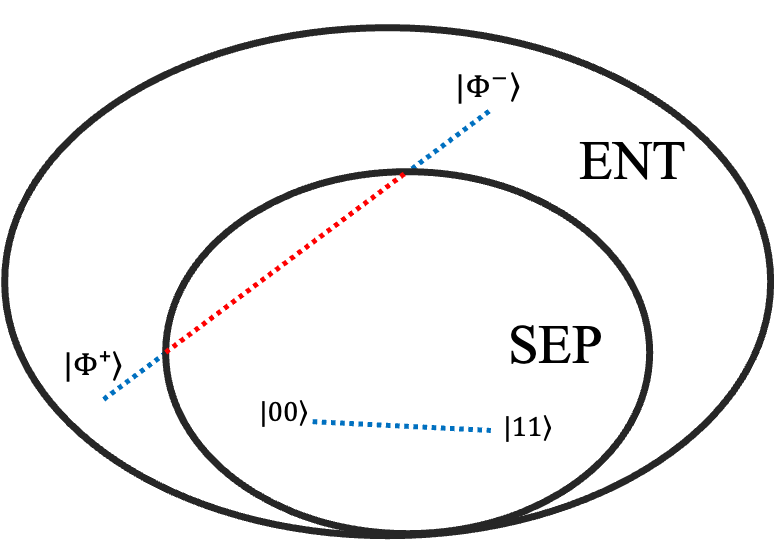
\includegraphics[width=0.45\textwidth]{image/L7_convexity.png}
            \end{figure}
            $\Rightarrow$ 즉, 전체 quantum state set에서 separable state는 \textit{convex set} 형태를 띄며, entangled state는 \textit{non-convex set}의 형태를 보인다.
        \end{frame}
        
        \begin{frame}
            \frametitle{Quantum channel: The mathematical structure behind EW}
            Alice가 maximally entangled state $\ket{\Phi^+}$를 준비하여 2번째 qubit을 Bob에게 quantum channel $\Lambda$를 통해 전송한다고 하자. 전체 system의 state는 다음과 같을 것이다.
            \begin{equation*}
                \rho^{AB} = [I \otimes \Lambda] (\ket{\Phi^+}\bra{\Phi^+})
            \end{equation*}
            이때, quantum channel을 통과하여 얻은 상태가 \textit{valid quantum state}가 되기 위해서 지켜야하는 성질은 다음과 같다. (CPTP)\\
            \vspace{0.2cm}
            \textbf{Completely Positive}\footnote{CP가 필요한 이유: measurement확률이 양수여야하기 떄문}
            \begin{itemize}
                \item positive ($\Lambda \ge 0$) : 연산 전후 positivity를 보존한다.
                \begin{equation*}
                    \forall \sigma \ge 0, \qquad \Lambda(\sigma) \ge 0.
                \end{equation*}
                \item k positive ($[I_k\otimes \Lambda]\ge 0.$) : $I$가 $k\times k$ matrix 일 때 positivity를 보존한다. (i.e., subsystem dim $k$에 대해 보존)
                \item \alert{completely positive} : $\forall k$에 대해 k positive
                $\Rightarrow$ $\Lambda$ is completely positive if $k \ge d$\footnote{$d$는 system의 차원}
            \end{itemize}
            \textbf{Trace Preserving}
            \begin{equation*}
                \text{tr} [\Lambda(A) = 1],\qquad \text{for }\text{tr}[A] = 1
            \end{equation*}
        \end{frame}

        \begin{frame}
            \frametitle{Quantum channel: The mathematical structure behind EW}
            \underline{Question}: 만약 quantum channel $\Lambda$가 P이지만 TP는 아닐때, \textbf{separable state}의 positivity는 보존되는가?\\
            \underline{Answer}: 보존된다! separable state는 두 system의 state의 곱으로 표현될 수 있기 때문에, 각각의 system에 따로 따로 연산을 취할 수 있기에 positivity를 보존할 수 있다.
            \begin{equation*}
                (I\otimes \Lambda) \sigma_{sep} = \sum_i p(i) \underbrace{\sigma^A_i}_{\ge 0} \otimes \underbrace{\Lambda(\sigma_i^B)}_{\ge 0 (\Lambda \ge 0)} \ge 0.
            \end{equation*}
            \vspace{-0.2cm}
            \begin{block}{Note}
                \begin{itemize}
                    \item separable state는 각 system에 대해 따로따로 연산을 취할 수 있기 때문에 CP condition을 필요로하지 않는다.(P를 만족하면 자동으로 CP도 만족한다.)\footnote{마치 classical mechanics의 system처럼}
                    \begin{equation*}
                        \text{if } \Lambda \ge 0,\quad \text{then } (I \otimes \Lambda) \ge 0. \qquad \Leftrightarrow \qquad \forall \sigma_{sep},\quad (I\otimes \Lambda)\sigma_{sep} \ge 0.
                    \end{equation*}
                    \item 반면 entangled state는 CP condition을 만족하지 않으면, 연산 결과 positivity가 보존되지 않는 경우가 존재한다. 
                    \begin{equation*}
                        \exists \Lambda,\ s.t.\ \text{ if } \Lambda \ge 0, \quad \text{but } (I \otimes \Lambda) \not \ge 0. \qquad \Leftrightarrow \qquad \exists \rho_{ent},\ s.t.\ \ (I\otimes \Lambda) \rho_{ent} \not \ge 0.
                    \end{equation*}
                \end{itemize}
            \end{block}
        \end{frame}

        \begin{frame}
            \frametitle{Another definition of entanglement using Channel}
            (idea) 앞에서 정의한 quantum channel의 성질을 이용하여 entangled state를 구분하는 방법을 다른 방식으로 정의할 수 있다. 
            \begin{definition}[(recap) entanglement]
                $\rho$가 entangled state라면, LOCC로 준비될 수 없다.
            \end{definition}
            \begin{definition}[entanglement on positivity]
                $\rho$가 entangled state라면, 다음을 만족하는 positive channel $\Lambda$가 존재한다. ($\exists \ \Lambda \ge 0$, but $I \otimes \Lambda \not ge 0$)
                \begin{equation*}
                    (I \otimes \Lambda) [\rho] \not \ge 0
                \end{equation*}
            \end{definition}
        \end{frame}

        \begin{frame}
            \frametitle{Another definition of EW using Channel}
            또한, 이를 이용하여 Entanglement Witness를 유도할 수 있다. 
            \begin{itemize}
                \item Quantum state $(I\otimes \Lambda)\rho$가 positive가 아니라는 뜻은, \textit{negative eigenvalue}를 가진다는 의미이다.
                \item 이는 다음을 만족하는 positive projector $Q$가 존재한다는 의미이다.\footnote{TODO}
                \begin{equation*}
                    \text{tr} [Q (I \otimes \Lambda)[\rho]] < 0 \qquad (equivalent) \qquad  \text{tr} [ (I \otimes \Lambda)^\dagger [Q] \rho] < 0
                \end{equation*}
                \item 위 식에서 $(I\otimes \Lambda)^\dagger[Q]$를 \alert{entanglement witness}로 정의할 수 있다. 
                \begin{equation*}
                    W \triangleq (I\otimes \Lambda)^\dagger[Q]
                \end{equation*}
            \end{itemize}
            \vspace{0.2cm}
            이제 $W$가 다음 2개의 성질을 만족하기 때문에 entanglement witness임을 보이고자한다.
            \begin{itemize}
                \item $\exists \rho_{ent}$ s.t. $\text{tr}[W\rho_{ent}] < 0$ $\rightarrow$ 자명하게 성립.
                \item $\forall \sigma_{sep}$ s.t. $\text{tr}[W\sigma_{sep}] \ge 0$
                성질 2번은 다음 관계에 따라 성립함을 입증할 수 있다.
                \begin{equation*}
                    \text{tr}[(I \otimes \Lambda)^\dagger [Q] \sigma_{sep}] = \text{tr}[\underbrace{Q}_{\ge 0} \underbrace{(I \otimes \Lambda)[\sigma_{sep}]}_{\ge 0}]
                \end{equation*}
            \end{itemize}
        \end{frame}

        \begin{frame}
            \frametitle{Choi-Jamiolkowski isomorphism}
            Map과 Bipartite operator간에는 어떤 \alert{관계}가 존재한다.
            \begin{itemize}
                \item map: 주어진 quantum state를 다른 state로 변환하는 linear operator ($\Lambda \ge 0$)
                \begin{equation*}
                    \Lambda \ : \ S(\mathcal H) \rightarrow S(\mathcal H)
                \end{equation*}
                \item bipartite operator: 2개의 system에 가해지는 operator
                \begin{equation*}
                    \mathcal X \in B(\mathcal H \otimes \mathcal H)
                \end{equation*}
            \end{itemize}
            
            $\Rightarrow$ \textit{Map $\Lambda$가 주어지면}, bipartite operator는 다음과 같이 특정 한 system에 map을 취하고 다른 system에는 아무런 연산도 하지 않는 것으로 표현할 수 있다.
            \begin{equation*}
                \mathcal X = (I \otimes \Lambda) [\ket{\Phi^+}\bra{\Phi^+}]
            \end{equation*}
            \begin{itemize}
                \item 만약 $\mathcal X \ge 0$이라면, $\Lambda$는 CP이며 $\mathcal X$는 valid quantum state가 된다.
                \item 만약 $\mathcal X \not \ge 0$이라면, $\Lambda$는 not CP이며 $\mathcal X$는 잘못된 mapping을 통해 얻은 EW이다.
            \end{itemize}
            \vspace{0.2cm}
            $\Leftarrow$ 반대로 \textit{operator $\mathcal X$가 주어지면}, $\Lambda$는 다음과 같이 표현할 수 있다.
            \begin{equation*}
                \Lambda [\sigma] = d \cdot \text{tr}_A [\sigma_A^T \mathcal{X}_{AB}] \ge 0
            \end{equation*} 
            \vspace{-0.6cm}
        \end{frame}

        \begin{frame}
            \frametitle{Choi-Jamiolkowski isomorphism}

            \begin{theorem}[Choi-Jamiolkowski isomorphism]
                Map과 bipartite operator\footnote{Choi matrix(operator), CJ operator, $\cdots$}는 one-to-one correspondence(i.e., isomorphism)를 가진다.
            \end{theorem}
            Example 1:
            \begin{itemize}
                \item map $\rightarrow$ operator : given map $D[\rho] = (\text{tr} \rho) \cdot I/d$
                \begin{align*}
                    \mathcal X &= (I\otimes D) [\ket{\Phi^+}\bra{\Phi^+}] = \frac{1}{d}\sum_{ij} \ket{i}\bra{j} \otimes \underbrace{D[\ket i \bra j] }_{\delta_{ij} \cdot I/d}\\
                                &= \frac{1}{d}\sum_i \ket i \bra i \otimes \frac{I}{d} = \frac{1}{d^2} I \otimes I.
                \end{align*}
                \item operator $\rightarrow$ map : given operator $\mathcal X = \frac{1}{d^2} I \otimes I$
                \begin{align*}
                    D[\sigma] &= d \cdot \text{tr}_A [\sigma_A^T \mathcal{X}_{AB}]  = d \cdot \text{tr}_A [\sigma_A^T \frac{1}{d^2} I_A \otimes I_B] \\
                            & = \frac{I_B}{d} \text{tr}[\sigma_A^T] = \frac{I}{d} \text{tr} [\sigma_A]
                \end{align*}
            \end{itemize}
        \end{frame}

        \begin{frame}
            \frametitle{Choi-Jamiolkowski isomorphism}
            Example 2: \textit{Identity} map $I[\rho] = \rho$에 대한 choi operator는?
            \begin{itemize}
                \item map $\rightarrow$ operator 
                \begin{align*}
                    \mathcal X &= (I\otimes I)[\ket{\Phi^+}\bra{\Phi^+}]  = \ket{\Phi^+} \bra{\Phi^+}
                \end{align*}
                \item operator $\rightarrow$ map
                \begin{align*}
                    I[\sigma] &= d \cdot \text{tr}_A [\sigma_A^T \mathcal{X}_{AB}]  \\
                                &= d^2 \cdot \text{tr}_{AA'}\Big[\sigma_{A'}\otimes \mathcal X_{AB} \ket{\Phi^+}_{AA'}\bra{\Phi^+}\Big] \qquad (\text{by } d\text{tr}_{A'}[\sigma_{A'} \ket{\Phi^+}_{AB}\bra{\Phi^+}] = \sigma_A^T) \\
                                &= d^2 \cdot \text{tr}_{AA'}\Big[\sigma_{A'}\otimes \ket{\Phi^+}_{AB}\bra{\Phi^+}\ket{\Phi^+}_{AA'}\bra{\Phi^+}\Big] = \sigma_B.
                \end{align*}
            \end{itemize}
            $\rightarrow$ 이는 \textit{quantum teleportation} 문제를 표현한다! \\
            (system $AB$가 $\mathcal X$를 공유, $AA'$에 대한 Bell 측정을 수행, $\sigma_{A'}$ state를 $\sigma_B$ state로 전달함)
            \begin{block}{Useful tips}\footnote{transpose를 없애려고 사용하는듯?}
                \vspace{-0.4cm}
                \begin{equation*}
                    d \text{tr}_A [\sigma_A \ket{\Phi^+}_{AB} \bra{\Phi^+}] = \sigma_B^T
                \end{equation*} 
                \begin{equation*}
                    d \text{tr}_A [\sigma_A^T \ket{\Phi^+}_{AB} \bra{\Phi^+}] = (\sigma_B^T)^T = \sigma_B
                \end{equation*} 
            \end{block}
        \end{frame}
    \end{section}

    %#################################### 
    \begin{frame}{Summary}
        \begin{block}{Summary}
            \begin{itemize}
                \item Quantum state SET 
                \begin{itemize}
                    \item Separable state들의 집합은 convex set.
                    \item Entangled state들의 집합은 non-convex set.
                \end{itemize}
                \item Quantum channel $\Lambda$
                \begin{itemize}
                    \item (positivity)
                    \begin{itemize}
                        \item 연산 대상이되는 system의 positivity를 보존하면 P
                        \item 전체 system의 positivity를 보존하면 CP
                        \item 전체 system의 positivity를 보존할 수 없으면 not CP
                    \end{itemize}
                    \item (channel) $(I \otimes \Lambda) \ge 0$ \& TP라면 $\Lambda$는 valid quantum channel로 사용할 수 있다.
                    \item (EW) $W \triangleq (I \otimes \Lambda)^\dagger [Q]$를 entanglement witness로 사용할 수 있다. 
                \end{itemize}
                \begin{equation*}
                    \begin{cases}
                        W = [I \otimes \Lambda] (\ket{\Phi^+} \bra{\Phi^+}) \not \ge 0 &\text{(not CP)} \\
                        \rho = [I \otimes \Lambda] (\ket{\Phi^+} \bra{\Phi^+}) \ge 0 &\text{(CP)}
                    \end{cases}
                \end{equation*}
            \item Choi-Jamiolkowski isomorphism
            \begin{itemize}
                \item map $\rightarrow$ operator
                \begin{equation*}
                    \mathcal X = (I \otimes \Lambda) [\ket{\Phi^+}\bra{\Phi^+}]
                \end{equation*}
                \item operator $\rightarrow$ map
                \begin{equation*}
                    \Lambda [\sigma] = d \cdot \text{tr}_A [\sigma_A^T \mathcal{X}_{AB}] \ge 0
                \end{equation*}
            \end{itemize}
            \end{itemize}
        \end{block}
    \end{frame}


    %#################################### 
    \begin{frame}{References}
        \begin{itemize}
            \item Lecture notes for EE547: Introduction to Quantum Information Processing (Fall 2024)
        \end{itemize}
        \vspace{6cm}
    \end{frame}


\end{document}